
\documentclass[letterpaper,10pt,onecolumn,titlepage]{article}

\usepackage{graphicx}                                        
\usepackage{amssymb}                                         
\usepackage{amsmath}                                         
\usepackage{amsthm}                                          

\usepackage{alltt}                                           
\usepackage{float}
\usepackage{color}
\usepackage{url}

%\usepackage{balance}
%\usepackage[TABBOTCAP, tight]{subfigure}
%\usepackage{enumitem}
\usepackage{pstricks, pst-node, pst-tree}


\usepackage{geometry}
\geometry{textheight=8.5in, textwidth=6in}

% random comment

\newcommand{\cred}[1]{{\color{red}#1}}
\newcommand{\cblue}[1]{{\color{blue}#1}}

\usepackage{hyperref}
\usepackage{geometry}

% please replace your name here...
\def\name{Jacob Branaugh}

\parindent = 0.0 in
\parskip = 0.2 in

%% The following metadata will show up in the PDF properties
\hypersetup{
  colorlinks = false,
  urlcolor = black,
  pdfauthor = {Jacob Branaugh},
  pdfkeywords = {cs472 ``computer architecture'' MIPS},
  pdftitle = {CS 472 Midterm 2},
  pdfsubject = {CS 472 Midterm 2},
  pdfpagemode = UseNone
}

\pagestyle{empty}
\begin{document}

\noindent {\large \bf Name: Jacob Branaugh \hfill CS/ECE 472/572 Midterm 2}

\noindent {\large \bf ID\#: 931-724-634}

%\emph{All answers should be typed directly below the questions. All work should be shown.
%  Answers with no work shown will be considered cheating. The exam should be typeset via
%  \LaTeX. All questions should be included in the exam. Yes, I am requiring that you do
%  this. It's good practice with \LaTeX, and you have an example as to how it should look
%  (see hw1.tex on the class website). Remove all of these notes from your final
%  submission.}
%
%\emph{This is an open book exam. As it is a take home exam, you are on the honor code.
%  Use your book, use your notes, don't use your friends.}
%
%\emph{There are 110 points possible on this exam.}
%
%\emph{Be detailed in your answers. Remember, this is a take home exam, so implied answers
%  will not be considered. Take the time and make everything explicit!}


\begin{enumerate}

\item (10 points) 9.23 \\
	When a CPU writes to the cache, both the item in the cache and the corresponding
	item in the memory must be updated. If data is not in the cache, it must be
	fetched from memory and loaded in the cache. If $t_{1}$ is the time taken to
	reload the cache on a miss, show that the effective average access time of the
	memory system is given by \\
	$t_{ave} = ht_{c} + (1-h)t_{m} + (1-h)t_{1}$

\item[\textbullet] Assuming the cache does not have to be reloaded, the average
	access time is equal to \\
	$t_{ave} = ht_{c} + (1-h)t_{m}$ \\
	In this case, the cache does take time to reload. For a single access, the time
	taken to reload the cache must be added to the no-miss access time. Since we are
	concerned about the average time, the cache reload time multiplied by the cache
	miss ratio must be added to the prior equation. This gives us \\
	$t_{ave} = ht_{c} + (1-h)t_{m} + (1-h)t_{1}$ \\
	which is the hit ratio multiplied by the cache access time plus the miss ratio
	multiplied the memory access time plus the miss ratio multiplied by cache reload
	time.

\item (10 points) 9.26 \\
	A system has a level 1 cache and a level 2 cache. The hit rate of the
	level 1 cache is 90\%, and the hit rate of the level 2 cache is 80\%. An access to
	level 1 cache requires one cycle, an access to level 2 cache requires four cycles,
	and an access to main memory requires 50 cycles. What is the average access time?
\item[\textbullet] The average access time can be expressed as a sum of the various access
	times multiplied by their respective occurrence rates: \\
	$t_{avg}=h_{1}t_{c1}+(1-h_{1})h_{2}t_{c2}+(1-h_{1})(1-h_{2})t_{m}$ \\
	where $h_{1}$ is the l1 cache hit rate, $h_{2}$ is the l2 cache hit rate, $t_{c1}$
	is the l1 cache access time, $t_{c2}$ is the l2 cache access time, and $t_{m}$ is
	the main memory access time. On average, the l1 cache access occurs as
	frequently as the l1 hit rate, the l2 cache access occurs as frequently as
	the l1 miss rate, and the main memory access occurs as frequently as the l2 miss
	rate and the l1 miss rate. Plugging in values gives: \\
	$t_{avg}=.9\times1+.1\times.8\times4+.1\times.2\times50=$ \textbf{2.22 cycles}

\item (10 points) 9.35 \\
	A 64-bit processor has an 8-MB, four-way set-associative cache with 32-byte lines.
	How is the address arranged in terms of set, line, and offset bits?
\item[\textbullet] With a four way set associative 8MB cache, each set will be 2MB in
	size. 32 byte lines means the number of lines will be $\frac{2^{30}}{2^{6}}$, or
	$2^{24}$. This means that 24 of the 64 bits will be required for the line number.
	Since the line size is 32 bytes, or $2^{6}$, 6 bits will be required for the line
	offset. Since the cache has four, or $2^{2}$, sets, 2 bits will be required for
	the set number.

\item (10 points) Assume a 64-bit virtual address and a 64-bit physical address. The page
	size is 4KB. How many total entries are there in the page table? Express your
	answer in powers of 2.
\item[\textbullet] The table is given as $4KB = 4*2^{10} = 2^{2}*2^{10} = 2^{12}$ bytes.
\item[\textbullet] Since the physical and virtual addresses are the same size, one address
	in ram and one address in the page table are the same size.
\item[\textbullet] A 64-bit address is equal to 8 bytes, or $2^{3}$ bytes.
\item[\textbullet] Therefore, the table can fit $\frac{2^{12}}{2^{3}}$, or \textbf{512}
	entries.

\item (10 points) 7.16  \\
	Derive an expression for the speedup ratio (i.e., the ratio of the execution time
	without pipelining to the execution time with pipelining) of a pipelined processor
	in terms of the number of stages in the pipeline \textit{m} and the number of
	instructions to be executed \textit{N}.
\item[\textbullet] $t_{no} = m \times N$ (each instruction executes sequentially)
\item[\textbullet] $t_{piped} = m + (N - 1)$ (the first instruction of m stages has to 
	finish, then an instruction of the remaining N-1 finishes every cycle)
\item[\textbullet] $S = \frac{t_{piped}}{t_{no}} = \frac{m+N-1}{mN}$

\item (10 points) 9.12 \\
	How is data in main store mapped on to each of the following?
	\begin{enumerate}
		\item[a)] Direct-mapped Cache: \\
			In a direct mapped cache, the main store is split into a number of
			equal sets, where each set is the size of the cache. From there,
			the sets are divided into lines, where the number of lines in the
			set is equal to the total number of lines in the cache.
		\item[b)] Fully-Associative Cache: \\
			In a fully associative cache, lines are taken from main memory and
			stored directly in cache. Each line's location is tagged with an
			address, and each line has an associated data validity bit.
		\item[c)] Set-Associative Cache: \\
			In a set associative cache, the cache is broken up into n sets for
			an n-way associative cache. A line has the same address across all
			n sets. When searching for an item, the sets are searched in
			parallel. When a match is found in any set, the search ends.
	\end{enumerate}

\item (10 points) 7.18 \\
	A processor executes an instruction in the following six stages. The time required
	by each stage in picoseconds is given for each stage.\\
	\\
	\begin{tabular}{ l l l }
		IF & Instruction Fetch & 300ps \\
		ID & Instruction Decode & 150ps \\
		OF & Operand Fetch & 250ps \\
		OE & Execute & 350ps \\
		 M & Memory Access & 700ps \\
		OS & Operand Store (writeback) & 200ps \\
	\end{tabular} \\

	\begin{enumerate}
		\item[a.] What is the time to execute an instruction if the processor is
			not pipelined? \\
			If the processor is not pipelined, each instruction will have to
			go through the whole fetch/execute process before the next can
			start. This gives the time to execute an instruction as: \\
			$300ps + 150ps + 250ps + 350ps + 700ps + 200ps =$ \textbf{1950ps}
		\item[b.] What is the time taken to fully execute an instruction assuming
			that this structure is pipelined in six stages and that there is an
			additional 20ps per stage due to the pipeline latches?\\
			If the processor is pipelined in six stages, the total time is
			equal to the total time from part a, but with an extra 20ps for
			each six stages (120ps total), or \textbf{2070ps}
		\item[c.] Once the pipeline is full, what is the average instruction
			rate?\\
			If the pipeline is full, an instruction will be completed every
			cycle. On average, the limiting factor will be the slowest cycle,
			with the addition of the time taken to latch the pipeline.
			Since the slowest cycle is the memory access at 700ps, an 
			instruction will be completed every \textbf{720ps}
		\item[d.] Suppose that 25\% of instructions are branch instructions that
			are taken and cause a 3 cycle penalty, what is the effective
			instruction execute time?\\
			Assuming the added conditions have carried through the problem,
			non branching instructions will take 720ps (from part c) and occur
			75\% of the time. Branching instructions will take an additional 3
			cycles on top of the existing instruction cycle, giving 720ps 4
			times (or 2880ps) occurring 25\% of the time. Averaging this
			gives\\
			$\frac{720+720+720+2880}{4} =$ \textbf{1260ps}
	\end{enumerate}

\item (10 points) 6.13 \\
	A computer has the following parameters:\\
	\\
	\begin{tabular}{ l r c }
		Operation & Frequency & Cycles \\
		\hline
		Arithmetic/logic instructions & 65\% & 1 \\
		     Register load operations & 10\% & 5 \\
		    Register store operations &  5\% & 2 \\
		      All branch instructions & 20\% & 8 \\
	\end{tabular} \\ \\
	If the average performance of the computer (in terms of its CPI) is to be
	increased by 20\% while executing the same instruction mix, what target
	must be achieved for the cycles per conditional branch instruction?
	\item[\textbullet] The CPI for branch instructions executed by machine A is as 
		follows: \\
		$CPI_{A} = \frac{freq_{ar}}{100} \times cyc_{ar} + 
			   \frac{freq_{ld}}{100} \times cyc_{ld} + 
			   \frac{freq_{st}}{100} \times cyc_{st} + 
			   \frac{freq_{br}}{100} \times cyc_{br}$ \\
		When values are plugged in, we get: \\
		$CPI_{A} = .65 + .5 + .1 + 1.6 = 2.85$ 
	\item[\textbullet] We know that a 20\% performance increase is desired. This means
		our new CPI will be equal to our old CPI multiplied by 1.2, or\\
		$CPI_{B} = \frac{CPI_{A}}{1.2} = 2.375$
	\item[\textbullet] If we reorder the equation from the first bullet for finding
		the branch instruction cycles using our new CPI, we get:\\
		$cyc_{br} = \frac{CPI_{B} - 
				  \frac{freq_{ar}}{100} \times cyc_{ar} - 
				  \frac{freq_{ld}}{100} \times cyc_{ld} - 
			  	  \frac{freq_{st}}{100} \times cyc_{st}}
				  {freq_{br}}$ \\
		Plugging values in gives us: \\
		$cycles_{branch} = \frac{2.375-.65-.5-.1}{.2} = 5.625$ \\
		We can only have integer multiples of clock cycles. Since 5.625 is our
		minimum target, 6 cycles will be too slow. This means that to see a 20\%
		performance increase, we need to see branch instructions being executed in 
		\textbf{5 cycles}

\item (15 points) 7.35 \\
	A RISC processor has an eight-stage pipeline: F D O E1 E2 MR MW WB (fetch, decode,
	register read operands, execute 1, execute 2, memory read, memory write, result
	writeback to register). Simple logical and arithmetic operations are complete by
	the end of E1. Multiplication is complete by the end of E2. How many cycles are
	required to execute the following code assuming that internal forwarding is not
	used?
	\begin{verbatim}
	(1) MUL   r0, r1, r2
	(2) ADD   r3, r1, r4
	(3) ADD   r5, r1, r6
	(4) ADD   r6, r5, r7
	(5) LDR   r1, [r2]
	\end{verbatim}
	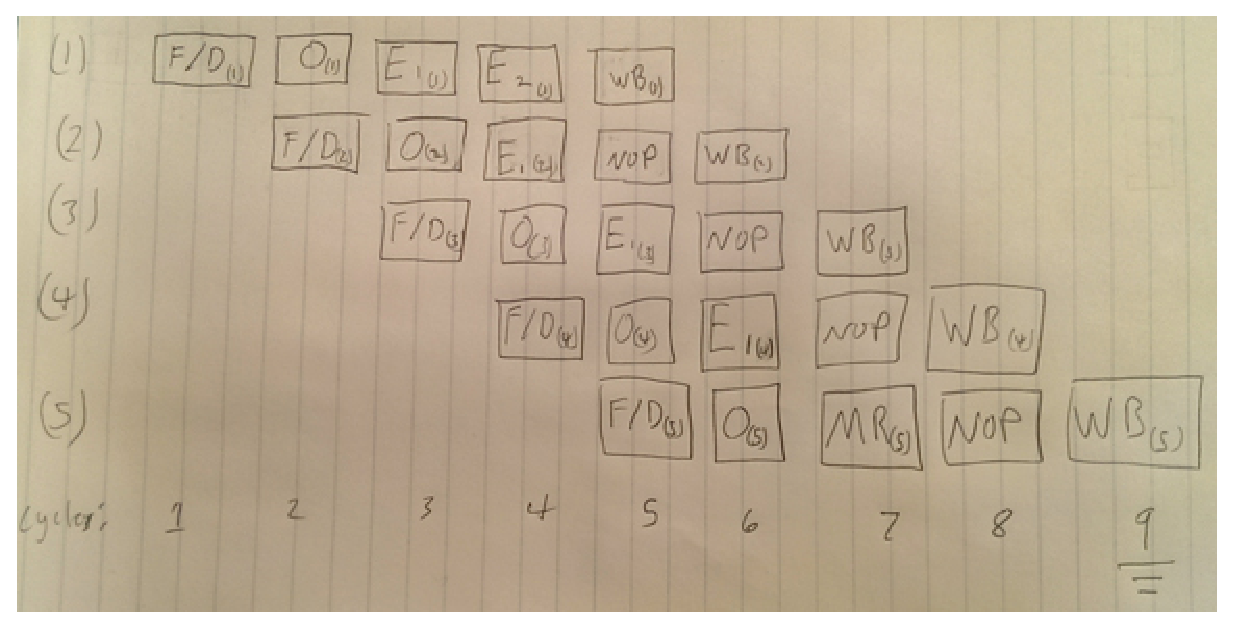
\includegraphics[width=5in]{7_35.eps}

%%%%%%%%%%%%%%%%%% NOT COMPLETE %%%%%%%%%%%%%%%%%%%%%%%%%%%%%%%%%%%%%%%%%%%%%%%%%%%%%%%%%%
\item (15 points) 7.38 \\
	the following table gives a sequence of instructions that are performed on a
	four-stage pipelined computer. Detect all hazards. For example, in instruction m
	uses operand r2 generated by instruction m-1, the write m-1,r2 in the RAW column
	in line m. \\
	\\
	\begin{tabular}{ c c c c c }
		Number & Instruction & RAW & WAR & WAW \\
		\hline
		1 & ADD r1, r2, r3 &   &   &   \\
		2 & ADD r4, r1, r3 &   &   &   \\
		3 & ADD r5, r1, r2 &   &   &   \\
		4 & ADD r1, r2, r3 &   &   &   \\
		5 & ADD r5, r2, r3 &   &   &   \\
		6 & ADD r1, r6, r6 &   &   &   \\
		7 & ADD r8, r1, r5 &   &   &   \\
	\end{tabular}\\
%%%%%%%%%%%%%%%%%%%%%%%%%%%%%%%%%%%%%%%%%%%%%%%%%%%%%%%%%%%%%%%%%%%%%%%%%%%%%%%%%%%%%%%%%%

\end{enumerate}

\end{document}

